
\section{Measurement set-up}
The measurements of the \gls{AVIS} are carried from within \Simulink model as shown in \figref{fig:avis:simulink:setup} and \figref{fig:avis:simulink:avis}.

\begin{figure}
\setlength\figurewidth{\columnwidth}
  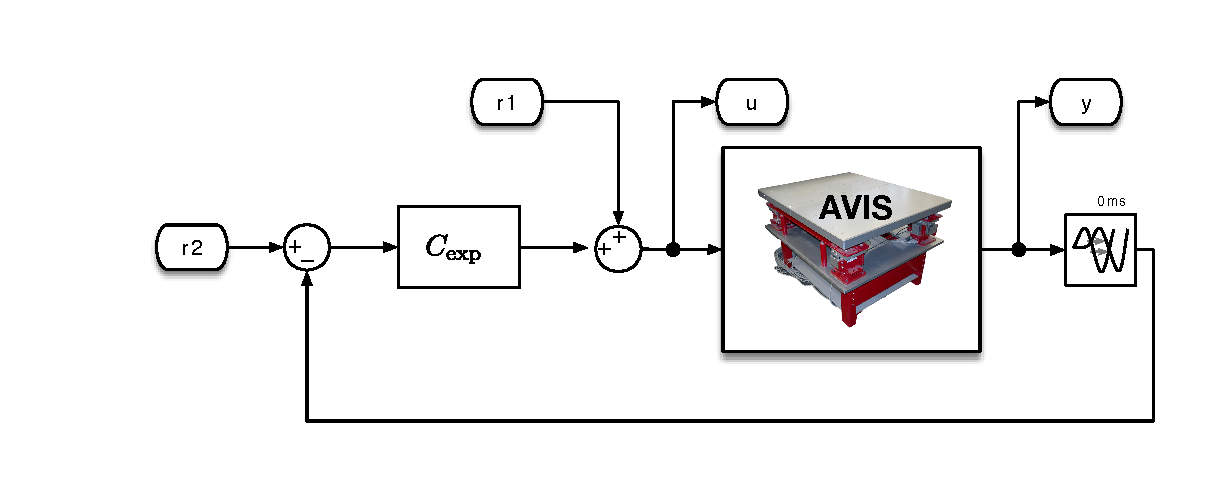
\includegraphics[width=\figurewidth]{\thisDir/figs/simulink-setup.pdf}
  \caption{Simulink model used during the AVIS measurements. All signals are six-dimensional real values.}
  \label{fig:avis:simulink:setup}
\end{figure}

In the top-level model (\figref{fig:avis:simulink:setup}), all signals are six-dimensional and each element corresponds to a single mechanical degree-of-freedom of the \gls{AVIS}, in order:
\begin{itemize}
  \item the translation in $x$ direction (horizontal),
  \item the translation in $y$ direction (horizontal),
  \item the translation in $z$ direction (vertical),
  \item the rotation along the $x$ axis,
  \item the rotation along the $y$ axis,
  \item the rotation along the $z$ axis.
\end{itemize}
In the main text, we have simplified this system to consider only the translation in the vertical direction (i.e. the third signal).
For the other directions, the applied signals (\code{r1} and \code{r2}) were set to $0$.
However, inside the feedback loop, all directions are controlled by the experimental controller $\experimental\Controller$.

Specifically, $\experimental\Controller$ is a $6\times6$ transfer function that is implemented as a discrete state-space model.
This controller was present beforehand~\citep{Rademakers2005MSc,vanderMaas2011MSc} and is given by the state-space matrices below
\begin{align}
  \experimental\Controller & \isdef \stateSpace{A}{B}{C}{D}\\
  A       &\approx 828.8 \cdot 10^{-3} \cdot \Identity{6} \\
  B = C &\approx \AvisMatrixDiagonal{93.83}{39.57} \cdot 10^{-3}\\
  D       &= \AvisMatrixDiagonal{4.982}{0.886} \cdot 10^{-3}
\end{align}
with $\Identity{n}$ the $n\times n$ identify matrix.
It can be seen that the controller is diagonal, i.e. the directions are decoupled, and that the dynamics are shared among the translational directions and the rotational direction respectively as shown in \figref{fig:avis:bodeplots:controllerAndSensor}.

\begin{figure}
\TODO{show bode plot of controller directions}
\caption{Bode plots of the $\experimental\Controller$ and sensor filter $F$.}
\label{fig:avis:bodeplots:controllerAndSensor}
\end{figure}

For multisine excitations the \code{RepeatingSequence} block was used to load the \code{r2} signal from \MATLAB, for noise excitations, the \code{RandomNumber} block of \Simulink was used instead.
The signals \code{r2}, \code{u} and \code{y} are returned from \Simulink to \MATLAB where further processing of the data is carried out.
This allows to compute the transfer function from \code{r2} to \code{u} and \code{y} respectively, or, the transfer function of the \gls{AVIS} block in the \Simulink model.

The \gls{AVIS} block (\figref{fig:avis:simulink:avis}), conceptually, contains:
\begin{itemize}
  \item a static decoupling $(K_{\mathrm{act}}, K_{\mathrm{sens}})$ of the physical \gls{AVIS} system, as derived in \citep{Rademakers2005MSc},
  \item logic to communicate with the Quanser Q8 \gls{DAQ} board which is physically connected to the \gls{AVIS}, and
  \item signal conditioning.
\end{itemize}

Specifically, the static decoupling of the \gls{AVIS} is given by the following gain matrices: \TODO{use pgfplotstable to add these matrices}
\begin{align}
  K_{\mathrm{act}}    &\approx \\
  K_{\mathrm{sens}} &\approx
\end{align}
Note that $K_{\mathrm{act}} \in \RR^{8\times6}$ and hence produces signals for the $8$ actuators on the \gls{AVIS}.
These signals are limited to the range $\pm 5\unit{V}$ before they are sent to the \glspl{DAC} on the Q8 \gls{DAQ} board to avoid overdriving the \glspl{DAC}.

The $6$ velocity signals that are read from the Q8 \gls{DAQ} are each filtered to \TODO{filtered such that what?} using a filter  $F$ with transfer function
\begin{equation}
  F(s) \approx \frac{6.51 s^2 + 122 s + 11.3}{6.4 s^2 - 16.6 s - 2.2}

\end{equation}
which is shown in \figref{fig:avis:bodeplots:controllerAndSensor}.
This filter is discretized automatically by \Simulink for the actual implementation, which happens in discrete time.

The output \code{y} is clipped to $\pm 20$ for easier detection of errors.
However, during normal operation and all the measurements, the signal levels were well within the linear region of this saturation block.

\begin{figure}
\setlength\figurewidth{\columnwidth}
  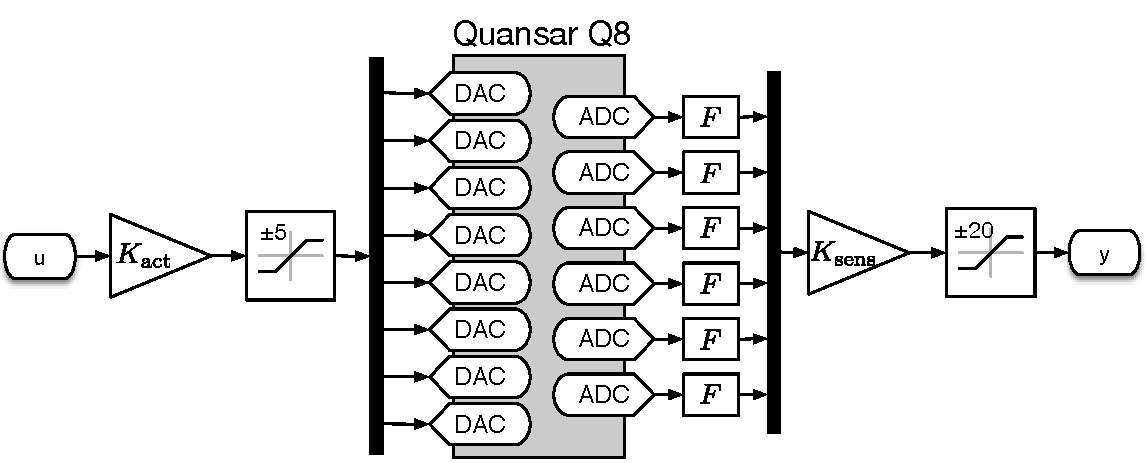
\includegraphics[width=\figurewidth]{\thisDir/figs/simulink-avis.pdf}
  \caption{Simulink model of the AVIS sub-block.}
  \label{fig:avis:simulink:avis}
\end{figure}

